% Options for packages loaded elsewhere
\PassOptionsToPackage{unicode}{hyperref}
\PassOptionsToPackage{hyphens}{url}
\documentclass[
]{article}
\usepackage{xcolor}
\usepackage{amsmath,amssymb}
\setcounter{secnumdepth}{-\maxdimen} % remove section numbering
\usepackage{iftex}
\ifPDFTeX
  \usepackage[T1]{fontenc}
  \usepackage[utf8]{inputenc}
  \usepackage{textcomp} % provide euro and other symbols
\else % if luatex or xetex
  \usepackage{unicode-math} % this also loads fontspec
  \defaultfontfeatures{Scale=MatchLowercase}
  \defaultfontfeatures[\rmfamily]{Ligatures=TeX,Scale=1}
\fi
\usepackage{lmodern}
\ifPDFTeX\else
  % xetex/luatex font selection
\fi
% Use upquote if available, for straight quotes in verbatim environments
\IfFileExists{upquote.sty}{\usepackage{upquote}}{}
\IfFileExists{microtype.sty}{% use microtype if available
  \usepackage[]{microtype}
  \UseMicrotypeSet[protrusion]{basicmath} % disable protrusion for tt fonts
}{}
\makeatletter
\@ifundefined{KOMAClassName}{% if non-KOMA class
  \IfFileExists{parskip.sty}{%
    \usepackage{parskip}
  }{% else
    \setlength{\parindent}{0pt}
    \setlength{\parskip}{6pt plus 2pt minus 1pt}}
}{% if KOMA class
  \KOMAoptions{parskip=half}}
\makeatother
\usepackage{longtable,booktabs,array}
\usepackage{calc} % for calculating minipage widths
% Correct order of tables after \paragraph or \subparagraph
\usepackage{etoolbox}
\makeatletter
\patchcmd\longtable{\par}{\if@noskipsec\mbox{}\fi\par}{}{}
\makeatother
% Allow footnotes in longtable head/foot
\IfFileExists{footnotehyper.sty}{\usepackage{footnotehyper}}{\usepackage{footnote}}
\makesavenoteenv{longtable}
\usepackage{graphicx}
\makeatletter
\newsavebox\pandoc@box
\newcommand*\pandocbounded[1]{% scales image to fit in text height/width
  \sbox\pandoc@box{#1}%
  \Gscale@div\@tempa{\textheight}{\dimexpr\ht\pandoc@box+\dp\pandoc@box\relax}%
  \Gscale@div\@tempb{\linewidth}{\wd\pandoc@box}%
  \ifdim\@tempb\p@<\@tempa\p@\let\@tempa\@tempb\fi% select the smaller of both
  \ifdim\@tempa\p@<\p@\scalebox{\@tempa}{\usebox\pandoc@box}%
  \else\usebox{\pandoc@box}%
  \fi%
}
% Set default figure placement to htbp
\def\fps@figure{htbp}
\makeatother
\setlength{\emergencystretch}{3em} % prevent overfull lines
\providecommand{\tightlist}{%
  \setlength{\itemsep}{0pt}\setlength{\parskip}{0pt}}
\usepackage{bookmark}
\IfFileExists{xurl.sty}{\usepackage{xurl}}{} % add URL line breaks if available
\urlstyle{same}
\hypersetup{
  hidelinks,
  pdfcreator={LaTeX via pandoc}}

\author{}
\date{}

\begin{document}

\section{Chronik der Familie Fleschutz (1412-1942)}\label{header-n0}

\textbf{Legende:} * = Geburt, ⚭ = Hochzeit, † = Tod, 🔨 = Beruf, 💥 =
Krieg, \{\} = Quelle. Die Chronik ist auch verfügbar im Format:
\href{Export/Chronik.docx}{.DOCX}, \href{Export/Chronik.epub}{.EPUB (für
E-Books)}, \href{Export/Chronik.html}{.HTML},
\href{Export/Chronik.odt}{.ODT}, \href{Export/Chronik.opml}{.OPML},
\href{Export/Chronik.pdf}{.PDF}, \href{Export/Chronik.rst}{.RST},
\href{Export/Chronik.rtf}{.RTF}, \href{Export/Chronik.tex}{.TEX},
\href{Export/Chronik.textile}{.TEXTILE}, sowie
\href{Export/Chronik.wiki}{.WIKI}.

\begin{longtable}[]{@{}ll@{}}
\toprule\noalign{}
Jahr & Ereignis \\
\midrule\noalign{}
\endhead
\bottomrule\noalign{}
\endlastfoot
1412 & Utz Brästel genannt Fläschuz, kauft die Güter zu "Wyler" und
"Mätzlins" (jetzt Fleschützen bei Börwang) vom Fürststift Kempten
\{\href{Quellen/Fuerststift_Kempten/Urkunde_263/}{Brief \& Urkunde
263}\} (erste urkundliche Erwähnung) \\
1480 & Jörg Fleschütz, Haldenwanger Pfarr. \\
1505 & Vergleich zwischen Hans Johann Fleschutz und Hans Caspar
Laubenberg \{\href{Quellen/Fuerststift_Kempten/Urkunde_1757/}{Urkunde
1757}\} \\
1516 & Frevelgerichtsbarkeit zu Fleschützen
\{\href{Quellen/Fuerststift_Kempten/Urkunde_2007/}{Urkunde 2007}\} \\
1525 & 💥 Deutscher Bauernkrieg, 200 Allgäuer Höfe wurden in Brand
gesteckt
\{\href{Quellen/Wikipedia/Deutscher_Bauernkrieg.pdf}{Wikipedia}\} \\
1530 & Georg Fleschutz (Hofmeister) kauft Wasserrecht zu Burkarts
\{\href{Quellen/Fuerststift_Kempten/Urkunde_2546/}{Urkunde 2546}\}, 1
Jahr später kauft er 2 Jauchert Acker
\{\href{Quellen/Fuerststift_Kempten/Urkunde_2566/}{Urkunde 2566}\}, 1540
kauft er ein Haus vom Konvent
\{\href{Quellen/Fuerststift_Kempten/Urkunde_2915/}{Urkunde 2915}\} und
1542 kauft er weitere 2 Häuser vom Konvent
\{\href{Quellen/Fuerststift_Kempten/Urkunde_2984}{Urkunde 2984}\} \\
1537 &
\pandocbounded{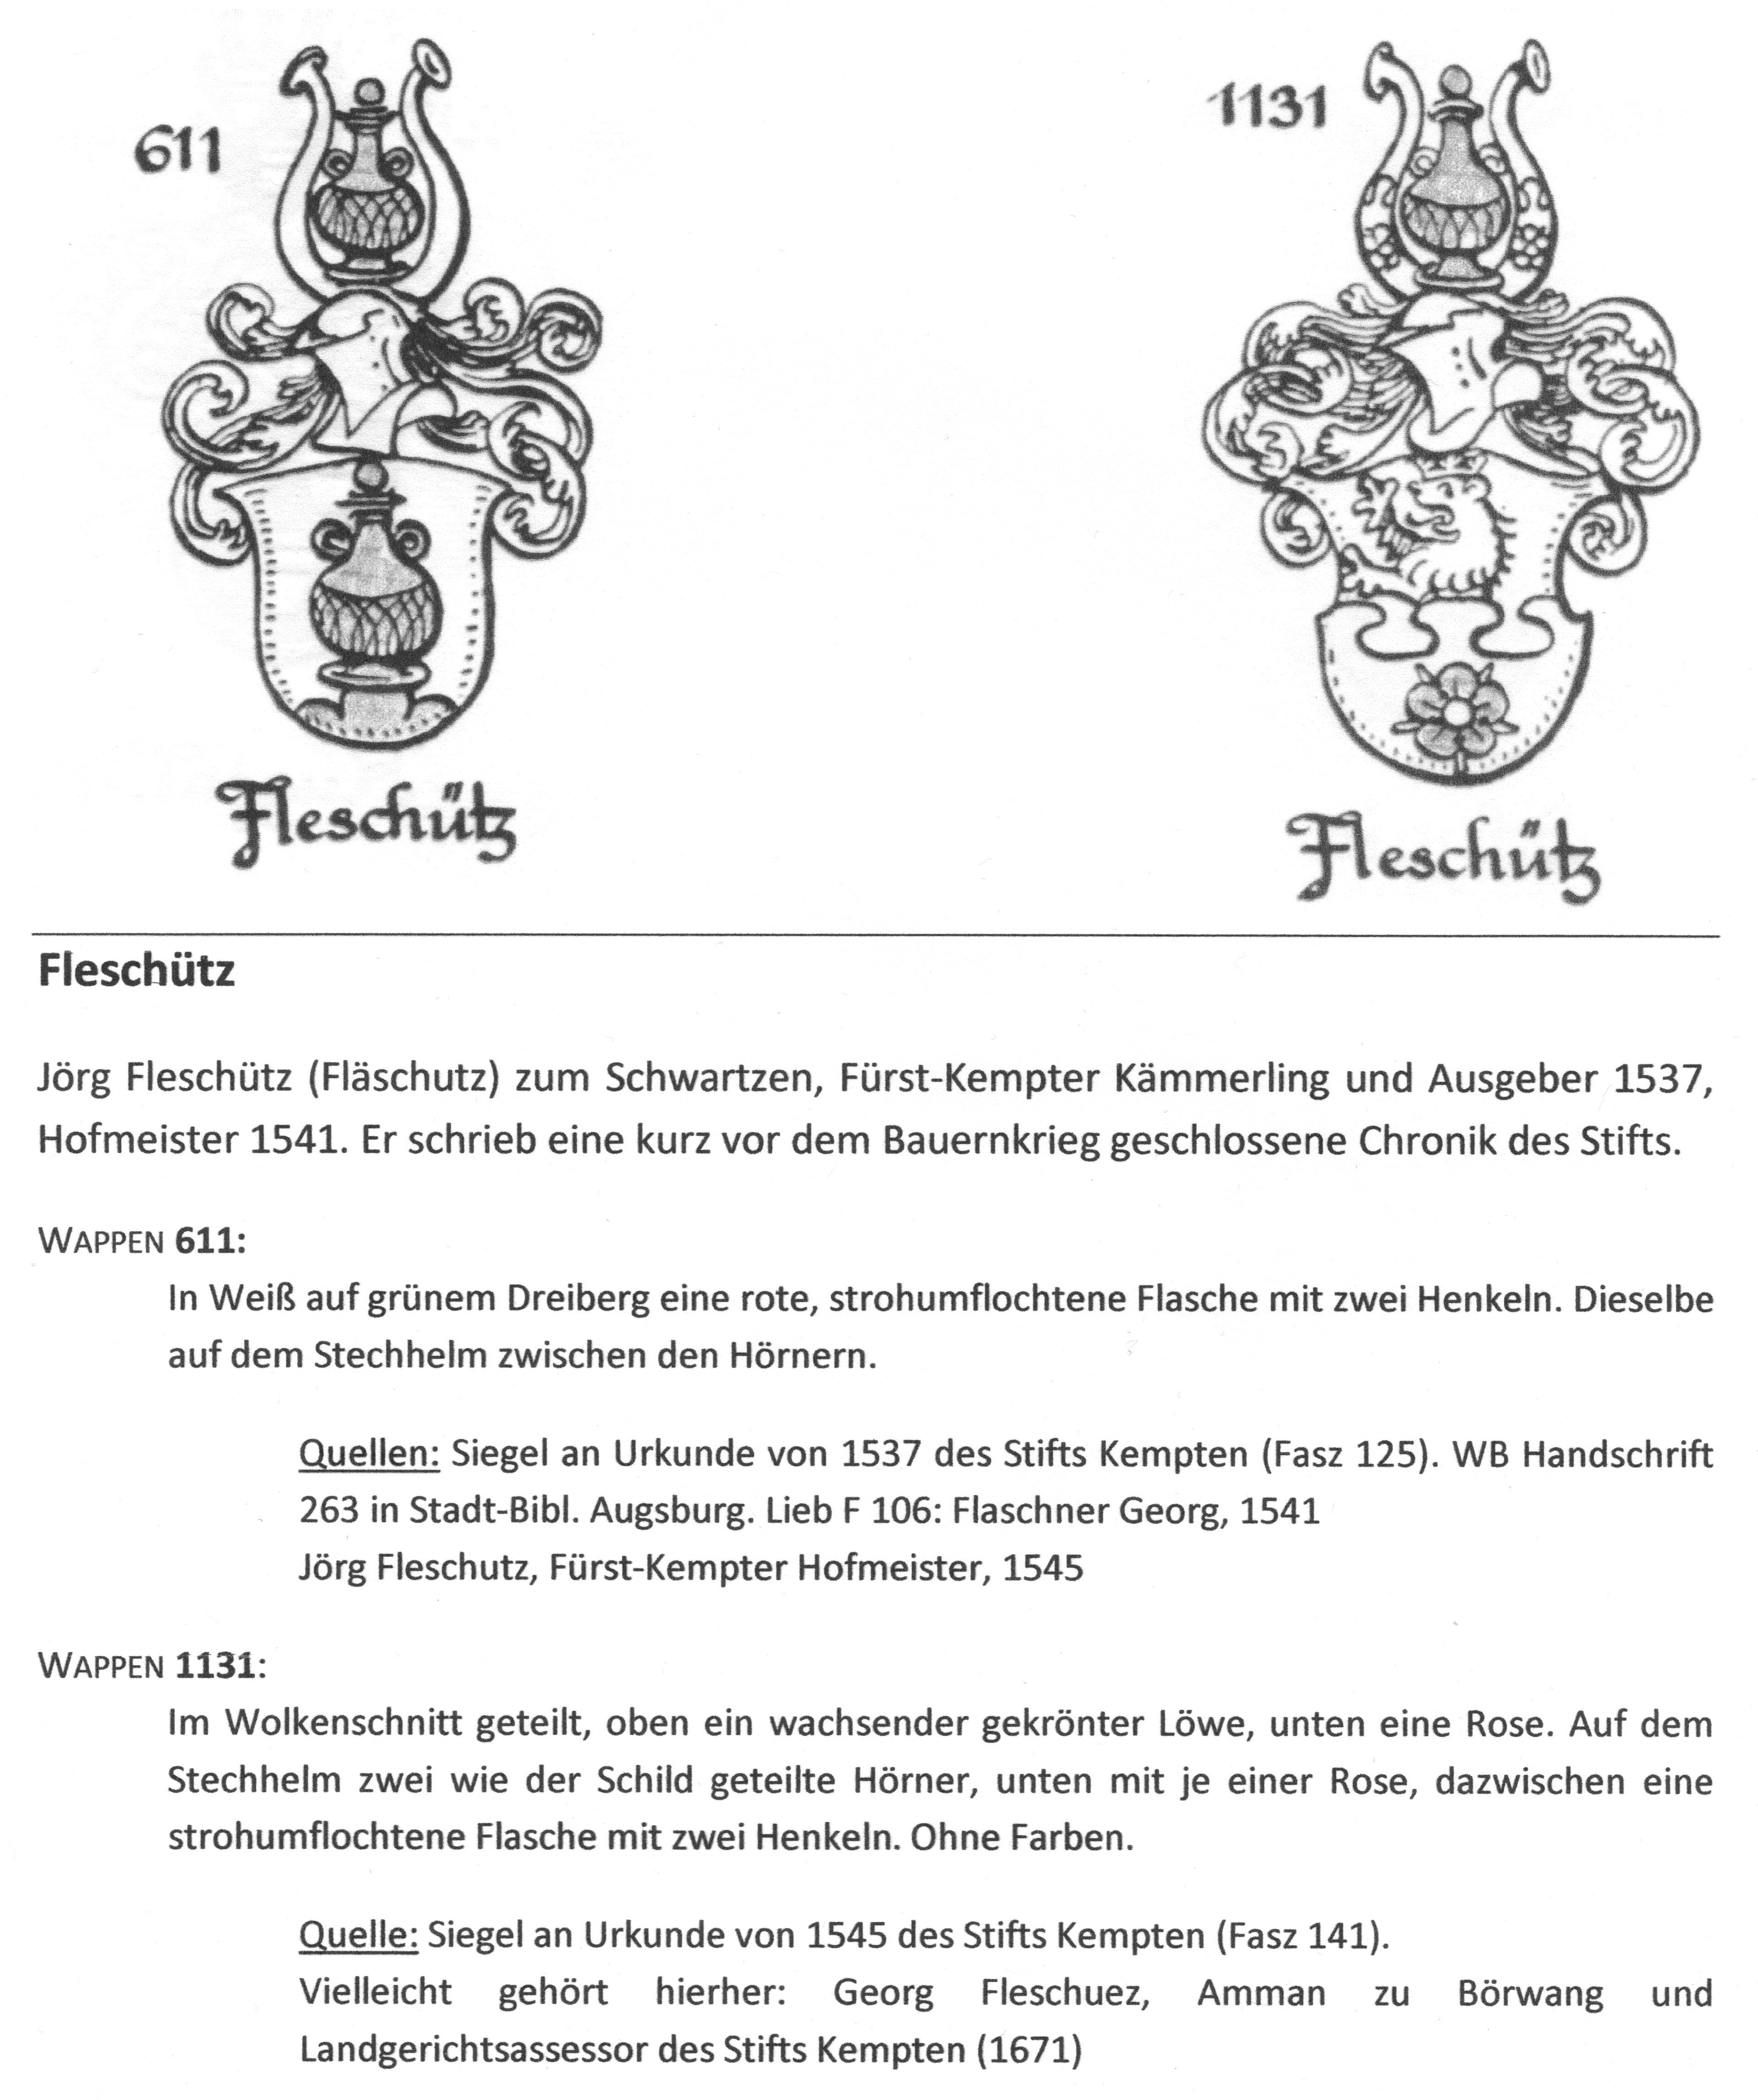
\includegraphics[keepaspectratio]{C:/Repos/Chronik/Quellen/Allgaeuer_Geschichtsfreund/Bildausschnitt.jpg}}
\{\href{Quellen/Allgaeuer_Geschichtsfreund/Wappen.pdf}{Allgäuer
Geschichtsfreund, Kempter Wappen und Zeichen}\} \\
1543 & Baltus Fleschutz, zum Weyler, genannt (bei den) Fleschutzen \\
1550 & Agatha Fleschutz verkauft ihr Gut zu Eschers (Untrasried) für 200
Gulden \{\href{Quellen/Fuerststift_Kempten/Urkunde_3316}{Urkunde
3316}\} \\
1550-1743 & Güter und Untertanen zu Fleschützen
\{\href{Quellen/Fuerststift_Kempten/Akte_1913}{Akte 1913}\} \\
1554 & Georg Fleschutz (in Schwarzen) wegen verliehener
Wirtschaftsgerechtsame
\{\href{Quellen/Fuerststift_Kempten/Urkunde_3495/}{Urkunde 3495}\} und
\{\href{Quellen/Fuerststift_Kempten/Urkunde_3499}{Urkunde 3499}\} \\
1564 & Baltasar Fleschutz (Scholare) will Priester werden \\
1565 & Christoph Fleschutz kauft ein Haus mit Taferngerechtigkeit
\{\href{Quellen/Fuerststift_Kempten/Urkunde_3800}{Urkunde 3800}\} \\
1565 & Balthus Fleschutz zu Fleschützen bekommt Zinsbrief von Lukas
Haini zu Bachtels
\{\href{Quellen/Fuerststift_Kempten/Urkunde_3778}{Urkunde 3778}\} \\
1618-1648 & 💥 Dreißigjähriger Krieg, dadurch Hungersnöte und Seuchen.
In Teilen Süddeutschlands überlebte nur ein Drittel der Bevölkerung
\{\href{Quellen/Wikipedia/Dreissigjaehriger_Krieg.pdf}{Wikipedia}\} \\
1658 & Hans Georg Fleschutz verkauft Baind zu Dickenbühl
\{\href{Quellen/Fuerststift_Kempten/Urkunde_5642/}{Urkunde 5642}\} \\
1666 & Baltasar Fleschutz, Bauschreiber im Stift Kempten \\
1686 & Georg Fleschutz zu Haubensteig kauft Weiderecht im Stadtallmey
\{\href{Quellen/Fuerststift_Kempten/Akte_1127/}{Akte 1127}\} \\
1791 &
\pandocbounded{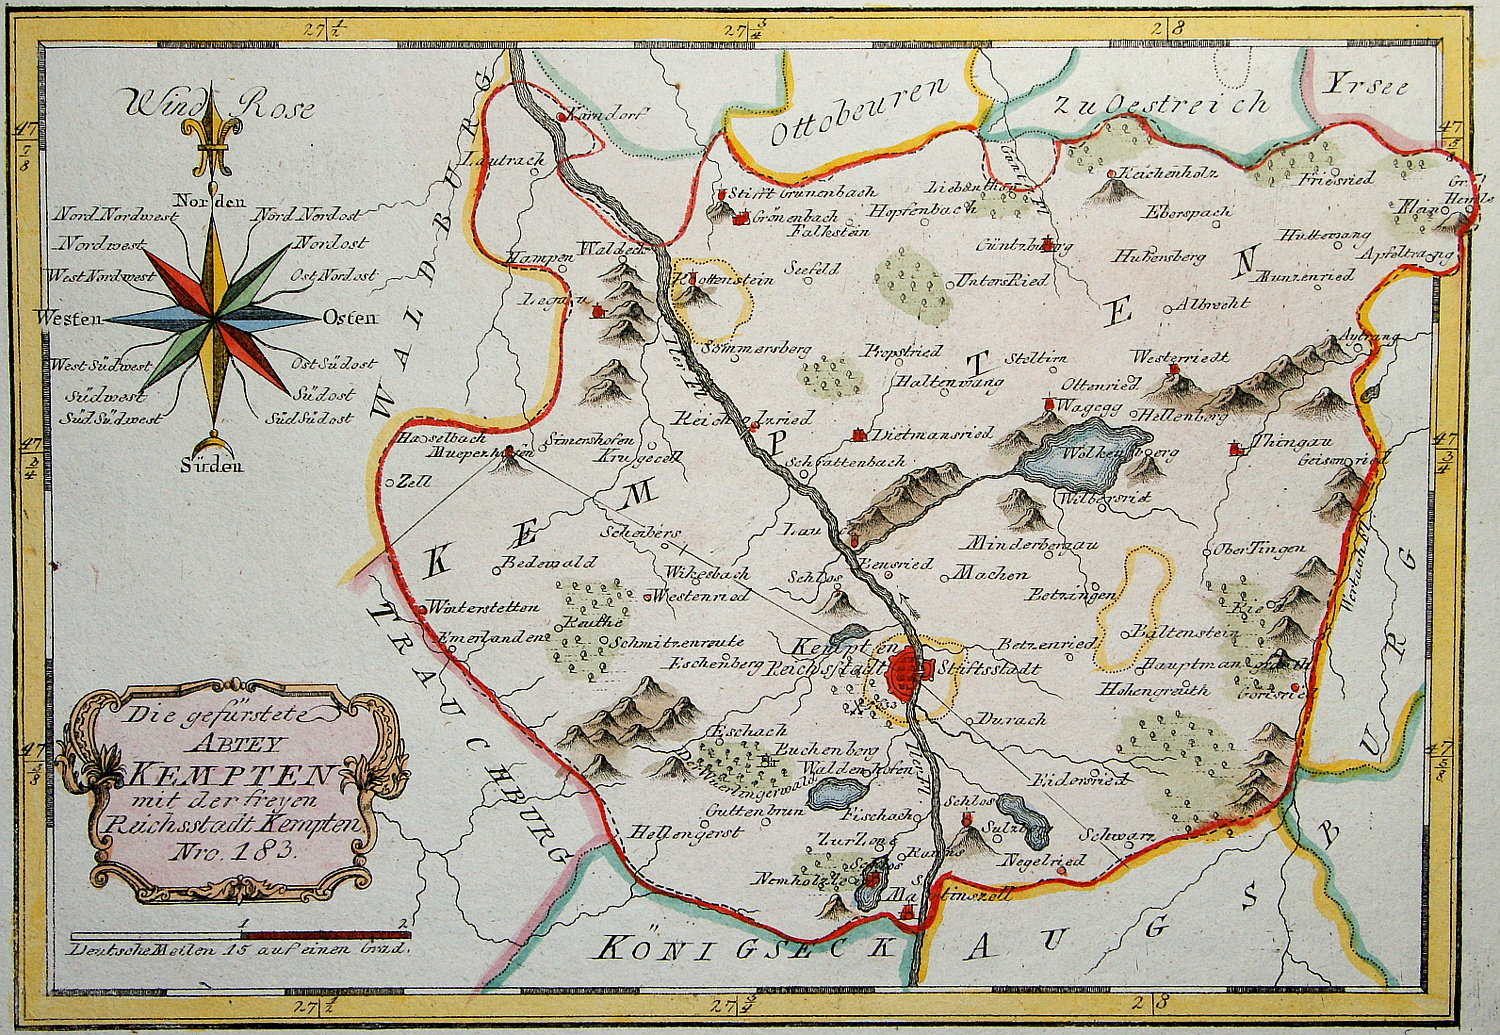
\includegraphics[keepaspectratio]{C:/Repos/Chronik/Quellen/Fuerststift_Kempten/1791_Karte.jpg}}
Karte des Territoriums der Fürstabtei Kempten von 1791
\{\href{Quellen/Wikipedia/Fuerststift_Kempten.pdf}{Wikipedia}\} \\
\end{longtable}

\begin{longtable}[]{@{}ll@{}}
\toprule\noalign{}
Vorname(n) & Ereignis \\
\midrule\noalign{}
\endhead
\bottomrule\noalign{}
\endlastfoot
\textbf{Baltasar} & †1646 ⚭Ursula Schneider
\{\href{https://data.matricula-online.eu/de/deutschland/augsburg/haldenwang-bei-kempten/1-S/?pg=1}{Sterberegister}\}
(vermutlich verwandt) \\
& \\
\textbf{Georg} & 🔨Hauptmann und Wirt ⚭1649 Sabina Brenberg(+1652) ⚭1654
Maria Heslin in Börwang
\{\href{https://data.matricula-online.eu/de/deutschland/augsburg/haldenwang-bei-kempten/1-S/?pg=9}{Sterberegister
Sabina}\}
\{\href{https://data.matricula-online.eu/de/deutschland/augsburg/haldenwang-bei-kempten/1-H/?pg=11}{Hochzeitsregister
mit Maria}\} (vermutlich verwandt) \\
& \\
& \textbf{Georg \& Sabina \& Maria\textquotesingle s Kinder:} (in
Börwang bei Haldenwang) \\
\textbf{Johann Georg} & ⚭1663 Maria Briechler in B.
\{\href{https://data.matricula-online.eu/de/deutschland/augsburg/haldenwang-bei-kempten/1-H/?pg=19}{Hochzeitsregister}\} \\
Maria & *1649 in B.
\{\href{https://data.matricula-online.eu/de/deutschland/augsburg/haldenwang-bei-kempten/1-T-1/?pg=10}{Taufregister}\}
(vermutlich verwandt) \\
Catharina & *1651 in B. +1654
\{\href{https://data.matricula-online.eu/de/deutschland/augsburg/haldenwang-bei-kempten/1-T-1/?pg=25}{Taufregister}\}
(vermutlich verwandt) \\
Ursula & *1655 in B.
\{\href{https://data.matricula-online.eu/de/deutschland/augsburg/haldenwang-bei-kempten/1-T-1/?pg=41}{Taufregister}\}
(vermutlich verwandt) \\
Elisabeth & *1656 in B.
\{\href{https://data.matricula-online.eu/de/deutschland/augsburg/haldenwang-bei-kempten/1-T-1/?pg=45}{Taufregister}\}
(vermutlich verwandt) \\
Regina & *1657 in B.
\{\href{https://data.matricula-online.eu/de/deutschland/augsburg/haldenwang-bei-kempten/1-T-1/?pg=51}{Taufregister}\}
(vermutlich verwandt) \\
Sabina & *1659 in B.
\{\href{https://data.matricula-online.eu/de/deutschland/augsburg/haldenwang-bei-kempten/1-T-1/?pg=57}{Taufregister}\}
(vermutlich verwandt) \\
& \\
& \textbf{Johann Georg \& Maria\textquotesingle s Kinder:} (in Börwang
bei Haldenwang) \\
Sabina & *1664 in B.
\{\href{https://data.matricula-online.eu/de/deutschland/augsburg/haldenwang-bei-kempten/1-T-1/?pg=72}{Taufregister}\} \\
Roman & *1665 in B.
\{\href{https://data.matricula-online.eu/de/deutschland/augsburg/haldenwang-bei-kempten/1-T-1/?pg=75}{Taufregister}\} \\
Rosina & *1666 in B.
\{\href{https://data.matricula-online.eu/de/deutschland/augsburg/haldenwang-bei-kempten/1-T-1/?pg=78}{Taufregister}\} \\
Ferdinand & *1667 in B.
\{\href{https://data.matricula-online.eu/de/deutschland/augsburg/haldenwang-bei-kempten/1-T-1/?pg=80}{Taufregister}\} \\
Anna & *1669 in B.
\{\href{https://data.matricula-online.eu/de/deutschland/augsburg/haldenwang-bei-kempten/1-T-2/?pg=4}{Taufregister}\} \\
Barbara & *1670 in B.
\{\href{https://data.matricula-online.eu/de/deutschland/augsburg/haldenwang-bei-kempten/1-T-2/?pg=7}{Taufregister}\} \\
Franz & *1671 in B.
\{\href{https://data.matricula-online.eu/de/deutschland/augsburg/haldenwang-bei-kempten/2-T/?pg=4}{Taufregister}\} \\
Maria & *1673 in B.
\{\href{https://data.matricula-online.eu/de/deutschland/augsburg/haldenwang-bei-kempten/2-T/?pg=7}{Taufregister}\} \\
Maria & *1675 in B.
\{\href{https://data.matricula-online.eu/de/deutschland/augsburg/haldenwang-bei-kempten/2-T/?pg=9}{Taufregister}\} \\
Franz & *1677 in B.
\{\href{https://data.matricula-online.eu/de/deutschland/augsburg/haldenwang-bei-kempten/2-T/?pg=12}{Taufregister}\} \\
Anna & *1679 in B.
\{\href{https://data.matricula-online.eu/de/deutschland/augsburg/haldenwang-bei-kempten/2-T/?pg=15}{Taufregister}\} \\
\textbf{Mang} & *1680 in B., ⚭1717 Anna Maria Geiger in B.
\{\href{https://data.matricula-online.eu/de/deutschland/augsburg/haldenwang-bei-kempten/2-T/?pg=12}{Hochzeitsregister}\} \\
Josef & *1681 in B.
\{\href{https://data.matricula-online.eu/de/deutschland/augsburg/haldenwang-bei-kempten/2-T/?pg=19}{Taufregister}\} \\
Georg & *1683 in B.
\{\href{https://data.matricula-online.eu/de/deutschland/augsburg/haldenwang-bei-kempten/2-T/?pg=22}{Taufregister}\} \\
& \\
& \textbf{Mang \& Anna Maria\textquotesingle s Kinder:} (in Börwang bei
Haldenwang) \\
Anna & *1718 in B.
\{\href{https://data.matricula-online.eu/de/deutschland/augsburg/haldenwang-bei-kempten/3-T/?pg=34}{Taufregister}\} \\
Anna Maria & *1719 in B.
\{\href{https://data.matricula-online.eu/de/deutschland/augsburg/haldenwang-bei-kempten/3-T/?pg=36}{Taufregister}\} \\
Ferdinand & *1721 in B.
\{\href{https://data.matricula-online.eu/de/deutschland/augsburg/haldenwang-bei-kempten/3-T/?pg=42}{Taufregister}\} \\
Johannes? & *1723 in B.
\{\href{https://data.matricula-online.eu/de/deutschland/augsburg/haldenwang-bei-kempten/3-T/?pg=45}{Taufregister}\} \\
\textbf{Josef} & *1725 in B. 🔨Bauer +06.04.1773 an böses Fieber in
Waizenried bei Untrasried ⚭11.08.1757 Anastasia Trunzer in Untrasried
\{\href{https://data.matricula-online.eu/de/deutschland/augsburg/haldenwang-bei-kempten/3-T/?pg=50}{Taufregister}\} \\
Dominik & *1726 in B.
\{\href{https://data.matricula-online.eu/de/deutschland/augsburg/haldenwang-bei-kempten/3-T/?pg=54}{Taufregister}\} \\
& \\
& \textbf{Josef \& Anastasia\textquotesingle s Kinder:} (auf Hof in
Waizenried 79 bei Untrasried, jetzt Schindele-Hof)
\{\href{https://data.matricula-online.eu/de/deutschland/augsburg/untrasried/16-FB/?pg=99}{Familienbuch}\} \\
Anna Barbara & *23.03.1758 in W. ⚭23.05.1793 mit Prack \\
Jakob & *23.07.1760 in W., †01.08.1760 mit nur 9 Tagen \\
\textbf{Leonhard} & *04.11.1761 in W. 🔨Bauer †09.03.1814 ⚭11.7.1785
Maria Adelheid Waldmann \\
Dominik & *08.10.1762 in W. +1762 \\
Maria Anna & *18.07.1764 in W. ⚭04.02.1788 mit Stehele \ldots{} nach
Mittelberg \\
Sabina & *26.10.1765 in W. †04.01.1766 mit nur 2 Monaten \\
Jakob & *06.07.1768 in W. \\
Afra & *06.08.1769 in W. †10.09.1769 mit nur 1 Monat \\
Theodor & *08.11.1770 \\
Anna Maria & *31.12.1772 in W. †18.08.1773 mit nur 7 Monaten \\
- & \textquotesingle+23.10.1773 (notgetauft) \\
Josef & *16.02.1775 in W. +09.03.1775 mit nur 21 Tagen \\
Franz Josef & *14.02.1776 \\
& \\
& \textbf{Leonhard \& Maria\textquotesingle s Kinder:} (auf Hof in
Waizenried 79 bei Untrasried, jetzt Schindele-Hof)
\{\href{https://data.matricula-online.eu/de/deutschland/augsburg/untrasried/16-FB/?pg=99}{Familienbuch}\} \\
Johann Georg & *07.07.1786 in W., †13.07.1786 \\
Anna Maria & *29.08.1787 in W. †04.09.1787 mit nur 6 Tagen \\
- & +24.09.1788 (notgetauft) \\
Genovefa & *03.01.1790 in W. †09.01.1790 mit nur 6 Tagen \\
\textbf{Johann Georg} & *20.04.1791 in W. 🔨Bauer †06.06.1865 ⚭ Maurus
... ⚭ Kreszentia Reichart \\
M. Afra & *05.08.1794 in W. \\
Ulrich & *04.07.1796 in W. †17.09.1861 in Burg ⚭Creszentia Hartmann,
*25.12.1791 \\
Franziska & *03.10.1797 in W. \\
Johann Baptist & \emph{23.06.1799 in W. †13.02.1875 in Engetried ⚭ Maria
Kreszenz Epp (}10.09.1798 †06.12.1862) \\
Maria Anna & *16.07.1805 in W. †1.7.1810 mit nur 5 Jahren \\
& \\
& \textbf{Johann Georg \& Maurus \& Kreszentia\textquotesingle s
Kinder:} (auf Hof in Waizenried 79 bei Untrasried, jetzt Schindele-Hof)
\{\href{https://data.matricula-online.eu/de/deutschland/augsburg/untrasried/16-FB/?pg=99}{Familienbuch}\} \\
Franz Xaver & *03.02.1818 in W. †06.02.1818 mit nur 3 Tagen \\
Maria Anna & *12.10.1819 in W. †14.07.1867 in Kraftisried? \\
Karolina & *16.03.1821 in W. \\
Franz Xaver & *13.05.1822 in W. †19.05.1822 mit nur 6 Tagen \\
Johann Georg & *14.08.1823 in W. †24.04.1830 \\
Johann ? & *02.08.1824 in W. †28.08.1824 mit nur 1 Monat \\
Ignaz & *31.07.1825 in W. †17.09.1825 mit nur 46 Tagen \\
M. Josefa & *31.10.1826 in W. \\
Johannes Chrysostomus & *09.02.1828 in W. †1907 in Obg. ⚭24.11.1862
Maria Antonia Schindele (zog als Privatier nach Obg.) \\
Johann L. & *24.06.1829 in W. †02.03.1830 \\
\textbf{Theresia} & *01.06.1831 in W. 🔨Privatiere †25.11.1901 in
Ostenried 71 bei Untrasried
\{\href{Quellen/Sterbebilder/1831_Theresia.jpg}{Sterbebild}\} \\
Theodor & *20.10.1832 in W. †1915 in Albrechts \\
Alois & *24.03.1834 \\
Johann Georg & *19.11.1835 in W. †03.04.1880 in Ostenried 71 \\
Johann Heinrich & *27.04.1837 in W. ⚭21.2.1881 in Altdorf mit Maria Anna
T. (2 Monate Hof, Trübsinn) \\
& \\
& \textbf{Theresia \& Xaver Prinz\textquotesingle s Kind}:
\{\href{https://data.matricula-online.eu/de/deutschland/augsburg/untrasried/16-FB/?pg=99}{Familienbuch}\} \\
\textbf{Johann Georg} & \emph{09.05.1868 in Ostenried 71 bei Untrasried
🔨Bauer †05.01.1933
\{\href{Quellen/Sterbebilder/1868_Georg.jpg}{Sterbebild}\} ⚭ Apollonia
Mayr (}09.02.1870 +08.12.1957
\{\href{Quellen/Sterbebilder/1870_Apollonia.jpg}{Sterbebild}\}) \\
& \\
& \textbf{Johann Georg \& Apollonia\textquotesingle s Kinder:} (zuerst
in Ostenried 71 bei Untrasried, dann in Albrechts 12 bei Günzach) \\
\textbf{Johann} & \emph{30.12.1895 in O. 🔨Bauer †29.05.1955 in
Albrechts \{\href{Quellen/Sterbebilder/1895_Johann}{Sterbebild}\} ⚭
Sophie Hartmann (}23.03.1904 †30.09.1977)
\{\href{Quellen/Sterbebilder/1904_Sophie.jpg}{Sterbebild}\} \\
Maria & *25.01.1897 in O. †05.01.1990 \\
Theresia & *27.04.1902 in O. †25.06.1987 ⚭Johann Kustermann \\
Georg & *19.04.1903 in O. †19.04.1903 mit nur 1 Tag \\
Johann Georg & *13.08.1906 in A. †09.05.1935 \\
Theodor & *10.12.1907 in A. 🔨Soldat †28.09.1942 bei Leningrad, Russland
\{\href{Quellen/Sterbebilder/1907_Theodor.jpg}{Sterbebild}\} \\
& \\
& 1914-1918 💥 1. Weltkrieg mit ca. 17 Millionen Toten
\{\href{Quellen/Wikipedia/Erster_Weltkrieg.pdf}{Wikipedia}\} \\
& 1939-1945 💥 2. Weltkrieg mit ca. 60-80 Millionen Toten
\{\href{Quellen/Wikipedia/Zweiter_Weltkrieg.pdf}{Wikipedia}\} \\
& \\
& \textbf{Johann \& Sophie\textquotesingle s Kinder:} (auf Hof in
Albrechts 12 bei Günzach) \\
Georg & *21.01.1935 in A., †19.03.1935 mit nur 2 Monaten \\
Amalie Maria Anna & *20.02.1936 in A. \\
Apollonia Theresia & *29.05.1937 in A. \\
Johann & *05.12.1938 in A. 🔨Bauer ⚭Rosmarie Höbel *18.12.1947 \\
Theodor Konrad & *12.11.1942 in A. 🔨Molkerei-Meister ⚭Sigrun Friede
*01.04.1949 in Radolfzell \\
\end{longtable}

\subsection{Danksagung}\label{header-n373}

Herzlichen Dank an alle die bei dieser Chronik mitgeholfen haben:

\begin{itemize}
\item
  An Karl Fleschutz und seinen Großvater für ihre Ahnenforschung und
  ihre Chronik der Familie Fleschutz in Burg.
\item
  An \href{https://data.matricula-online.eu/de/}{Matricula Online}, die
  die vielen Kirchenbücher in Europa eingescannt haben.
\item
  An Bernhard für die Sterbebilder und an Jörg für den Hinweis zu
  Matricula Online.
\item
  An Andrea für das schwierige Entziffern der Handschriften.
\end{itemize}

\end{document}
